\documentclass[aspectratio=169]{beamer}
\usepackage{import}
\usepackage{algpseudocode}
\subimport{../../latex/}{setup_presentation}

\algrenewcommand\algorithmicdo{\textcolor{violet}{do}}
\algrenewcommand\algorithmicwhile{\textcolor{violet}{while}}
\algrenewcommand\algorithmicend{\textcolor{violet}{end}}
\algrenewcommand\algorithmicif{\textcolor{violet}{if}}
\algrenewcommand\algorithmicthen{\textcolor{violet}{then}}



\title{ECE 780 To 8 Project}
\subtitle{Bug Algorithms using Neural Networks}
\author{Andreas Stöckel}
\date{July 24th, 2017}

\setbeamertemplate{footline}[frame number]


\begin{document}

\begin{frame}[plain,noframenumbering]
	\centering
	{\Large\color{violet}{\inserttitle}\\}
	{\large\color{violet}{\insertsubtitle}\\[0.5cm]}
	{\large{\insertauthor}\\[0.25cm]}
	Computational Neuroscience Research Group\\
	Centre for Theoretical Neuroscience\\[0.25cm]
	
\includegraphics[width=0.3\textwidth]{media/uwlogo.pdf}\\[0.25cm]
	\insertdate
\end{frame}

% Overview:
% - Motivation
% - What are bug algorithms?
%	- "Sensor based planning"
%   - Require local information only
%   - Can be shown to work optimally
%   - Which are the assumptions?
%   - Algorithm <==> Implementation

\begin{frame}{Motivation}

\begin{columns}
	\column{0.6\textwidth}
	\begin{itemize}
		\setlength{\itemsep}{0.4cm}
		\item<1-> In class, we mostly talked about path planning using \emph{\color{violet}{global}} information.
		\item<1-> Often, robotic and biological agents alike are restricted to \emph{\color{violet}local}, \emph{\color{violet}sensor-based} information.
		\item<2-> \emph{\color{violet}Bug algorithms} (Lumelsky and Stepanov 1987)\\
		are a simplistic class of local planing algorithms/policies.
		\item<3->[$\leadsto$] Can these algorithms be implemented in a biological, neural substrate?
	\end{itemize}
	\column{0.4\textwidth}
	\centering
	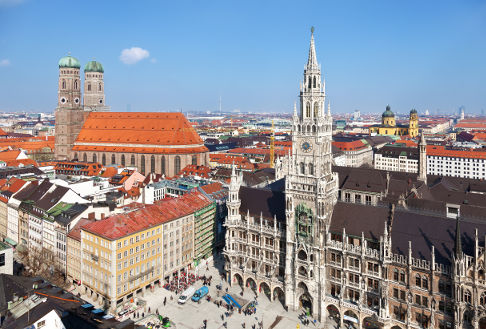
\includegraphics[width=0.9\textwidth]{media/munich_small.jpg}\\
	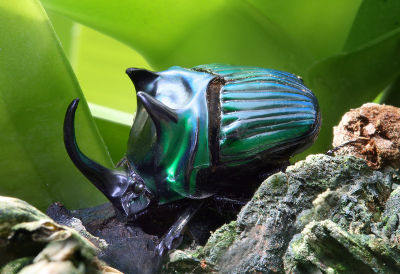
\includegraphics[width=0.9\textwidth]{media/bug_small.jpg}\\
	\footnotesize\color{aluminium4}Source: Wikimedia Commons
\end{columns}

\end{frame}

%\begin{frame}[plain,noframenumbering]{Outline}
%	\begin{itemize}
%		\setlength{\itemsep}{0.4cm}
%		\item Motivation
%		\item Bug Algorithms
%		\item Spiking Neural Networks and the Neural Engineering Framework
%		\item Implementation and Results
%	\end{itemize}
%\end{frame}

\begin{frame}[plain,noframenumbering]
\centering
{\Large\textcolor{violet}{\textsc{PART I}}}\\
\huge Bug Algorithms
\end{frame}

\begin{frame}{Bug Algorithm Assumptions}
	\begin{columns}[c]
			\column{0.65\textwidth}
				\emph{\textcolor{violet}{Environment}}
				\begin{itemize}
					\setlength{\itemsep}{0.2cm}
					\item Start location $\vec p_\mathrm{start}$, goal location $\vec p_\mathrm{goal}$
					\item Polygonal obstacles $O_1, \ldots, O_n$
				\end{itemize}\vspace{0.3cm}
				\only<2->{\emph{\textcolor{violet}{Robot}}}~
				\begin{itemize}
					\setlength{\itemsep}{0.2cm}
					\item<2-> Knows direction towards goal (absolute and relative)
					\item<4-> Knows the straight line distance to the goal
					\item<5-> Has no knowledge of obstacles (no map)
					\item<6-> Has a contact sensor
					\item<7-> Moves in straight lines or along obstacle boundaries
					\item<8-> Has memory to store distances and angles
				\end{itemize}
			\column{0.35\textwidth}			
			\includegraphics<1>[width=\textwidth]{media/assumptions_sketch_start_goal_obstacle.pdf}
			\includegraphics<2>[width=\textwidth]{media/assumptions_sketch_absolute_angle.pdf}
			\includegraphics<3>[width=\textwidth]{media/assumptions_sketch_relative_angle.pdf}
			\includegraphics<4>[width=\textwidth]{media/assumptions_sketch_distance.pdf}
			\includegraphics<5>[width=\textwidth]{media/assumptions_sketch_question.pdf}
			\includegraphics<6>[width=\textwidth]{media/assumptions_sketch_contact.pdf}
			\includegraphics<7->[width=\textwidth]{media/assumptions_sketch_boundaries.pdf}
	\end{columns}
\end{frame}

\videoframe{media/video/demo_bug_direct_success.mp4}

\videoframe{media/video/demo_bug_direct_fail.mp4}

\videoframe{media/video/demo_bug_0_success.mp4}

\begin{frame}{The Bug 0 algorithm}
	\begin{columns}[c]
		\column{0.6\textwidth}
		\begin{minipage}{\textwidth}\begin{algorithmic}[1]
			\While{not at goal}
				\State{move towards the goal}
				\If{hit an obstacle}
					\While{not able to move towards the goal}
						\State{follow obstacle boundary \emph{CCW}}
					\EndWhile
				\EndIf
			\EndWhile
		\end{algorithmic}\end{minipage}
		\vspace{0.5cm}
		\begin{itemize}
			\item[\color{chameleon3}$\oplus$] Algorithm solely depends on goal direction
			\item[$\ominus$] The algorithm may fail...
		\end{itemize}
		\column{0.4\textwidth}
		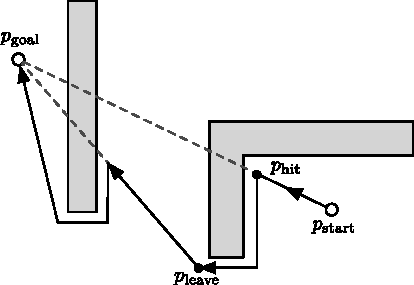
\includegraphics[width=\textwidth]{media/bug_0_sketch.pdf}\\
		\footnotesize\textcolor{aluminium4}{Source: Lectures on Robotic Planning and Kinematics, Bullo and Smith, 2016}
	\end{columns}
\end{frame}

\videoframe{media/video/demo_bug_0_fail.mp4}

%\begin{frame}{Bug 0: Distance plot}
%	\centering
%	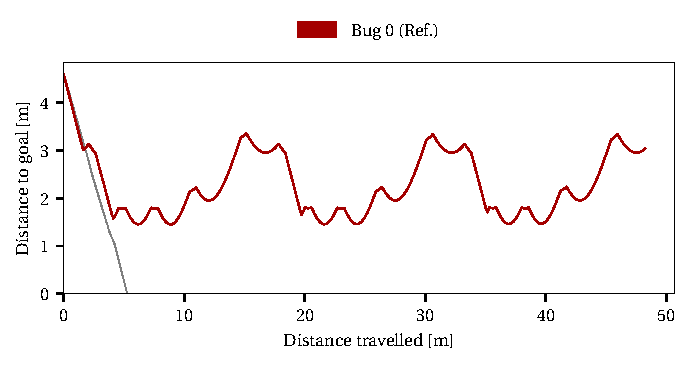
\includegraphics{media/vis_dist_map_demo_03_bug_0_ref.pdf}
%\end{frame}

\begin{frame}{The Bug 2 algorithm}
	\begin{columns}
		\column{0.6\textwidth}
		\begin{minipage}{\textwidth}\begin{algorithmic}[1]
				\State{$\alpha \gets$ goal direction}
				\While{not at goal}
				\State{move towards the goal}
				\If{hit an obstacle}
					\State{$d_\mathrm{hit} \gets$ distance to goal}
					\While{distance to goal $\geq d_\mathrm{hit}$ \textcolor{violet}{and}\\\hspace{2.13cm}goal direction $\neq \alpha$}
						\State{follow obstacle boundary}
					\EndWhile						
				\EndIf
				\EndWhile
		\end{algorithmic}\end{minipage}
		\vspace{0.25cm}
		\begin{itemize}
			\item[\color{chameleon3}$\oplus$] If $\vec p_\mathrm{goal}$ is reachable from $\vec p_\mathrm{start}$, the algorithm will find a path
			\item[$\ominus$] Not always better than Bug 1
		\end{itemize}
		\column{0.4\textwidth}
		\centering
		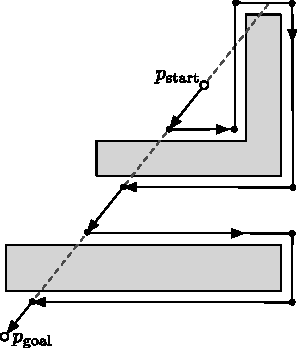
\includegraphics[width=0.75\textwidth]{media/bug_2_sketch.pdf}\\
		\raggedright
		\footnotesize\textcolor{aluminium4}{Source: Lectures on Robotic Planning and Kinematics, Bullo and Smith, 2016}
	\end{columns}
\end{frame}

\videoframe{media/video/demo_bug_2.mp4}

%\begin{frame}{Bug 2: Distance plot}
%	\centering
%	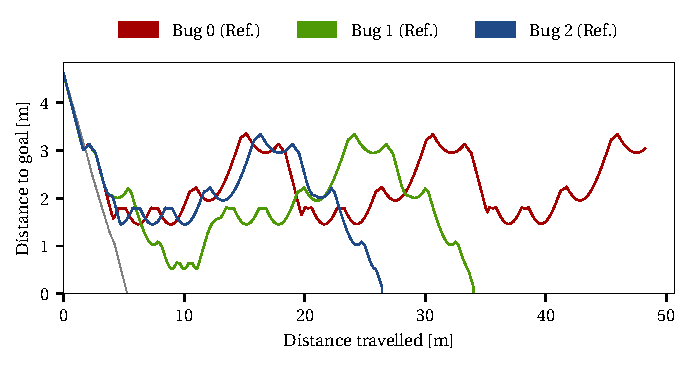
\includegraphics{media/vis_dist_map_demo_03_bug_0_ref_bug_1_ref_bug_2_ref.pdf}
%\end{frame}

\begin{frame}[plain,noframenumbering]
	\centering
	{\Large\textcolor{violet}{\textsc{PART II}}}\\
	\huge Spiking Neural Networks and\\the Neural Engineering Framework
\end{frame}

\begin{frame}{Textbook Biological Model Neuron}
	\centering
	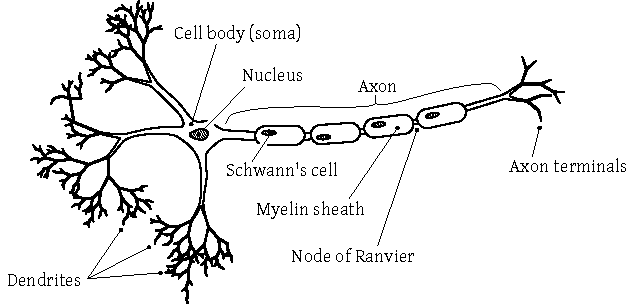
\includegraphics{media/neuron_sketch.pdf}\\
\end{frame}

\begin{frame}{Leaky Integrate and Fire Neuron}
	\centering
	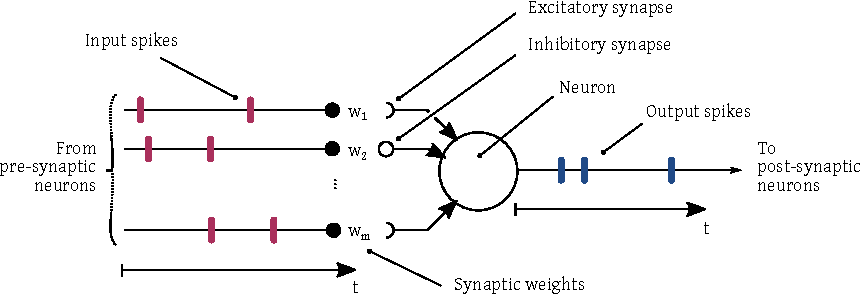
\includegraphics[scale=0.9]{media/spiking_neuron.pdf}
	\begin{itemize}
		\item Input spikes induce current $J$ in cell body
		\item Cell body modelled as dynamical system in continuous time
		\begin{align*}
			\tau \dot u(t) &= J - u(t) & u(t) &\gets 0 \text{ if } u(t) = 1
		\end{align*}
		\item<2->[\symbolfont{⚠}] Not your usual artificial neural network! Intrinsic dynamics! Spike noise!
	\end{itemize}
\end{frame}

\begin{frame}{The Neural Engineering Framework (NEF)}
	\centering
	\begin{columns}[T]
		\column{0.7\textwidth}
		\begin{itemize}
			\setlength{\itemsep}{0.25cm}
			\item Systematic way of building spiking neural networks
			\item \emph{\textcolor{violet}{Principle 1:}}\\
			Populations of spiking neurons represent $\vec x$
			\item \emph{\textcolor{violet}{Principle 2:}}\\
			Connections between populations compute $f(\vec x) = \vec y$
			\item \emph{\textcolor{violet}{Principle 3:}}\\
			Self-connections implement dynamics $\mathrm{d}/\mathrm{d}t\, \vec x = g(\vec x)$
		\end{itemize}
		\centering
		\vspace{0.25cm}
		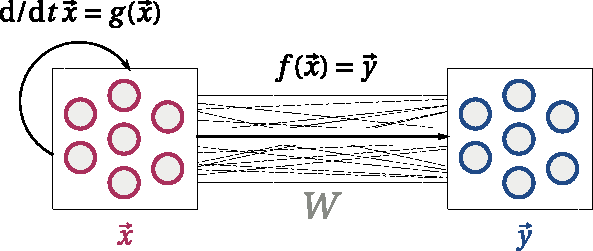
\includegraphics[scale=0.7]{media/nef_principles.pdf}
		\column{0.3\textwidth}
		\centering
		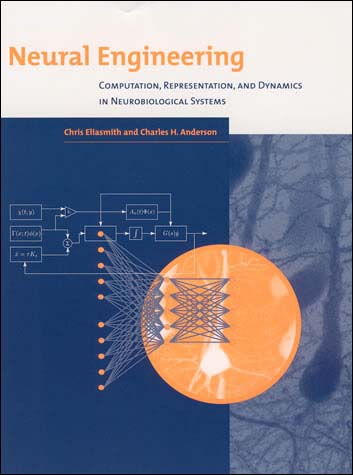
\includegraphics[width=0.95\textwidth]{media/nef_book.jpg}\\[0.1cm]
		\raggedright
		\footnotesize{\color{aluminium4}Chris Eliasmith and\\ Charles H.~Anderson,\\Neural Engineering, 2003}
	\end{columns}
\end{frame}

\begin{frame}{Nengo}
	\begin{itemize}
		\item Nengo: Python software implementation of the NEF, available on GitHub\\ \footnotesize\textcolor{aluminium4}{(Bekolay et al., Nengo: A Python tool for building large-scale functional brain models,\\Frontiers in Neuroinformatics, 2014)}
	\end{itemize}
	\vspace{0.1cm}
	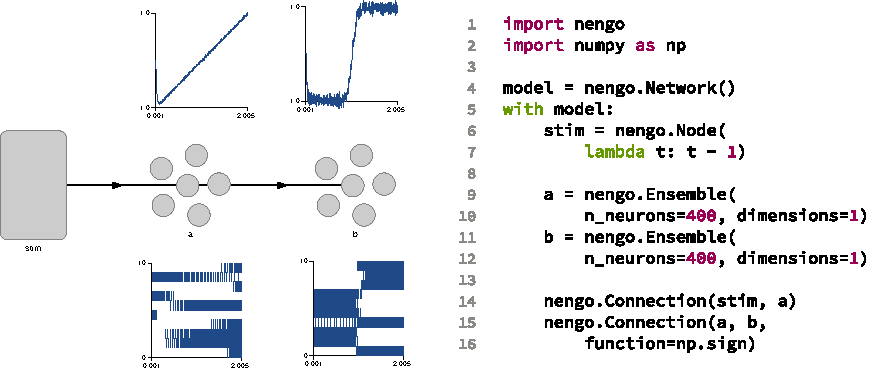
\includegraphics[width=\textwidth]{media/nengo_example.pdf}
\end{frame}

\begin{frame}[plain,noframenumbering]
\centering
{\Large\textcolor{violet}{\textsc{PART III}}}\\
\huge Implementation and Results
\end{frame}

\begin{frame}{Simulator Environment}
	\begin{columns}[t]
		\column{0.3\textwidth}
		\emph{\textcolor{violet}{Body \& Environment}}
		\begin{itemize}
			\item Discrete simulation $\Delta t = 10\,\mathrm{ms}$
			\item Disk-shaped robot
			\item Robot slides along obstacles
		\end{itemize}
		\centering
		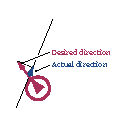
\includegraphics[width=0.9\textwidth]{media/assumptions_sketch_slide.pdf}
		\column{0.35\textwidth}
		\emph{\textcolor{violet}{Sensors}}
		\begin{itemize}
			\item Distance $d$, contact sensor
			\item Absolute and relative orientation (unit vectors $\vec \alpha_\mathrm{a}$, $\vec \alpha_\mathrm{r}$)
			\item Radar for obstacle boundary following
		\end{itemize}
		\centering
		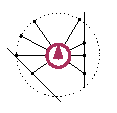
\includegraphics[width=0.85\textwidth]{media/radar_1.pdf}
		\column{0.3\textwidth}
		\emph{\textcolor{violet}{Motor System}}
		\begin{itemize}
			\item Non-holonomic 2-DOF drive
			\item Relative control vector $\vec v = (v_\mathrm{x}, v_\mathrm{y})$
		\end{itemize}
		\vspace{0.35cm}
		\centering
		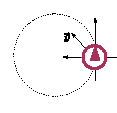
\includegraphics[width=0.9\textwidth]{media/motor.pdf}
	\end{columns}
\end{frame}

\begin{frame}{Basic Behaviours: Move Towards Goal \& Follow Obstacle}
	\begin{columns}[t]
		\column{0.5\textwidth}
		\emph{\textcolor{violet}{Move Towards Goal}}\\
		\begin{itemize}
			\item Connect relative direction vector $\vec \alpha_r$ to the motor control output $\vec v$
		\end{itemize}
		\vspace{1.5cm}
		\centering
		
\includegraphics[width=0.85\textwidth]{media/move_goal_direction.pdf}
		\column{0.5\textwidth}
		\emph{\textcolor{violet}{Follow Obstacle}}\\
		\begin{itemize}
			\item Rotate radar vectors by $\approx 45°$
			\item Weighted sum of radar vectors; smaller distance, more weight
		\end{itemize}
		\centering
		\includegraphics<1>[width=0.65\textwidth]{media/radar_1.pdf}
		\includegraphics<2>[width=0.65\textwidth]{media/radar_2.pdf}
		\includegraphics<3>[width=0.65\textwidth]{media/radar_3.pdf}
	\end{columns}
\end{frame}

\videoframe{media/video/demo_bug_follow.mp4}

\begin{frame}{Bug 0: Reference Implementation}
	\centering
	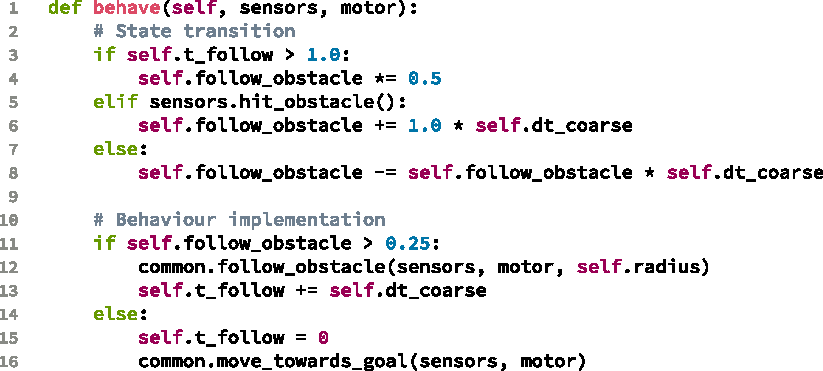
\includegraphics{media/bug_0_ref_code.pdf}
\end{frame}

\begin{frame}{Bug 0: Neural Network}
	\centering
	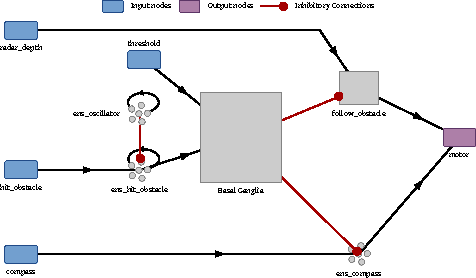
\includegraphics[height=0.775\textheight]{media/nengo_bug_0_network.pdf}
\end{frame}

\videoframe{media/video/bug_0_comparison.mp4}

\begin{frame}{Bug 0: State over Time}
	\centering
	\includegraphics<1>[height=0.85\textheight]{media/sim_1_traj_map_04_bug_0_neural_bug_0_ref.pdf}
	\includegraphics<2>{media/sim_1_trace_map_04_Bug_0_ref.pdf}
	\includegraphics<3>{media/sim_1_trace_map_04_Bug_0_neural.pdf}
\end{frame}

\begin{frame}{Bug 0: Distance Plot}
	\centering
	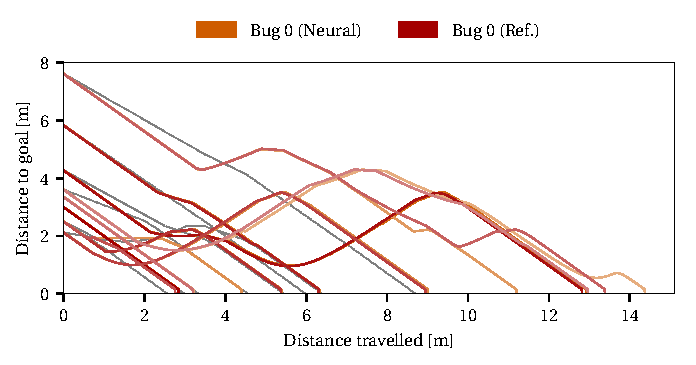
\includegraphics{media/vis_dist_map_04_bug_0_neural_bug_0_ref.pdf}
\end{frame}

\begin{frame}{Bug 2: Thinking About States}
		\begin{columns}[T]
		\column{0.6\textwidth}
		\begin{minipage}{\textwidth}\begin{algorithmic}[1]
				\State{$\alpha \gets$ goal direction}
				\While{not at goal}
				\State{move towards the goal}
				\If{hit an obstacle}
				\State{$d_\mathrm{hit} \gets$ distance to goal}
				\While{distance to goal $\geq d_\mathrm{hit}$ \textcolor{violet}{and}\\\hspace{2.13cm}goal direction $\neq \alpha$}
				\State{follow obstacle boundary}
				\EndWhile						
				\EndIf
				\EndWhile
		\end{algorithmic}\end{minipage}
		\vspace{0.5cm}
		\begin{itemize}
			\item<1->\emph{\textcolor{violet}{Simulator/Neural network:}}\\
			Executes algorithm \enquote{tick-wise}
			\item[$\leadsto$] Translate to state machine
		\end{itemize}
		\column{0.4\textwidth}
		\only<2->{\emph{\color{violet}States:}}~
		\begin{enumerate}[1.]
			\item<2-> \texttt{MEM\_DIR}: Memorize direction
			\item<2-> \texttt{MOVE}: Move towards goal
			\item<2-> \texttt{MEM\_DIST}: Memorize distance
			\item<2-> \texttt{FOLLOW}: Follow obstacle outline
		\end{enumerate}
		\vspace{0.5cm}
		\only<3->{\emph{\color{violet}State Transition Table:}}~
		\begin{align*}
			\only<3->{\epsilon &\rightarrow 1, & 1 &\rightarrow 2, & 2 &\rightarrow 3, & 4 &\rightarrow 2} \vphantom{1234}
		\end{align*}
		\vspace{0.2cm}
		\begin{itemize}
			\item<4->[$\leadsto$] How to implement this as a spiking neural network?
		\end{itemize}
	\end{columns}
\end{frame}

\begin{frame}{Bug 2: State Transition Network}
	\centering
	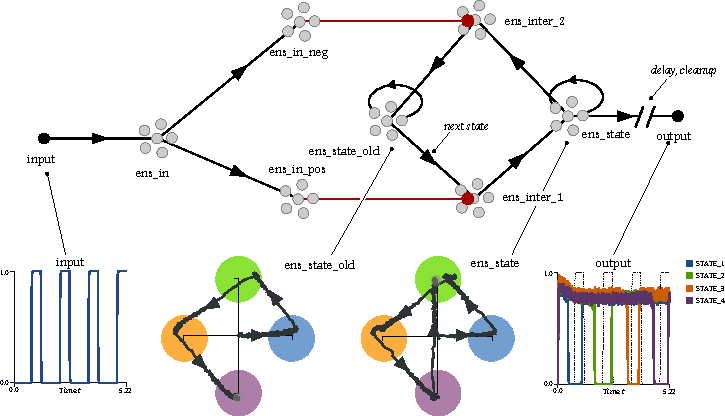
\includegraphics{media/nengo_state_network.pdf}
\end{frame}

\videoframe{media/video/bug_2_comparison.mp4}

\begin{frame}{Bug 2: State over Time}
	\centering
	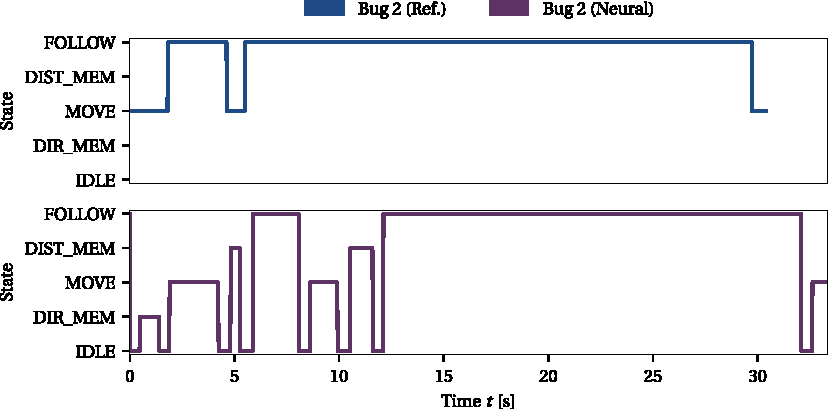
\includegraphics{media/vis_trace_map_demo_03_bug_2_ref_bug_2_neural.pdf}
\end{frame}

\begin{frame}{Bug 2: Distance Plot}
	\centering
	\includegraphics<1>{media/vis_dist_map_demo_03_bug_2_neural_bug_2_ref.pdf}
%	\includegraphics<2>{media/vis_dist_t_map_demo_03_bug_2_neural_bug_2_ref.pdf}
\end{frame}

\begin{frame}{Conclusion}
	\begin{columns}[t]
		\column{0.5\textwidth}
		\emph{\textcolor{violet}{Biological Plausibility}}
		\begin{itemize}
			\item Given the sensors, neurobiological implementation plausible, only few thousand neurons required
			\item Many of the sensors map to biological systems:
			\begin{itemize}
				\item radar $\leftrightarrow$ structure from motion
				\item contact $\leftrightarrow$ tactile sensors
				\item distance and direction $\leftrightarrow$ olfactory system in insects
			\end{itemize}\vspace{0.225cm}
			\item[\symbolfont{⚠}] Yet, the given implementation must not be seen as a biological model!
		\end{itemize}
		\column{0.5\textwidth}
		\only<2->{\emph{\textcolor{violet}{Lessons}}}~
		\begin{itemize}
			\item<2-> Implementing the simulator:\\doing CG right is hard\textellipsis
			\item<2-> Implementation of \textcolor{violet}{\emph{Bug 0}} as neural network quite trivial and works well.
			\item<2-> Implementation of \textcolor{violet}{\emph{Bug 2}} suffers from noise/chaotic behaviour.
		\end{itemize}
		\vspace{0.3cm}
		\only<3->{\emph{\textcolor{violet}{Challenges}}}~
		\begin{itemize}
			\item<3-> Plenty of magic constants in both reference and neural implementation
			\item<3-> State transition network
		\end{itemize}
	\end{columns}
\end{frame}

\begin{frame}[plain,noframenumbering]
	\centering
	\huge
	Thank you for your attention!
\end{frame}


%\begin{frame}[allowframebreaks]
%	\frametitle{References}
%	\bibliographystyle{amsalpha}
%	\bibliography{../../../../bibliography/bibliography.bib}
%\end{frame}

\appendix

\backupbegin
\begin{frame}{The Bug 1 algorithm}
\begin{columns}
	\column{0.6\textwidth}
	\begin{minipage}{\textwidth}\begin{algorithmic}[1]
			\While{not at goal}
			\State{move towards the goal}
			\If{hit an obstacle}
			\State{\textcolor{violet}{at the same time}}
			\State{\hspace{0.5cm}circumnavigate the obstacle}
			\State{\hspace{0.5cm}track minimum distance to goal}
			\State{follow boundary back to minimum}
			\EndIf
			\EndWhile
	\end{algorithmic}\end{minipage}
	\vspace{0.5cm}
	\begin{itemize}
		\item[\color{chameleon3}$\oplus$] One can show that this algorithm is \emph{\textcolor{violet}{complete}}
		\item[$\ominus$] Relatively complex, paths are far from optimal
	\end{itemize}
	\column{0.4\textwidth}
	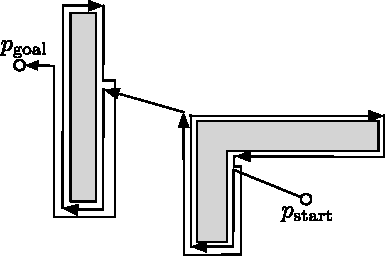
\includegraphics[width=\textwidth]{media/bug_1_sketch.pdf}\\
	\footnotesize\textcolor{aluminium4}{Source: Lectures on Robotic Planning and Kinematics, Bullo and Smith, 2016}
\end{columns}
\end{frame}

\videoframe{media/video/demo_bug_1.mp4}

%\begin{frame}{Bug 1: Distance plot}
%	\centering
%	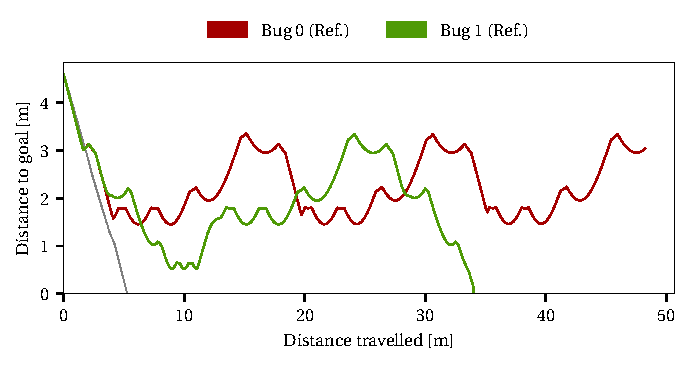
\includegraphics{media/vis_dist_map_demo_03_bug_0_ref_bug_1_ref.pdf}
%\end{frame}
\begin{frame}{Spiking Neural Networks: Why Bother?}
	\begin{itemize}
		\item<1-> Can implement linear algebra and dynamical systems in spiking neural networks\\
		\item<2->[$\Rightarrow$] Why not just use the mathematical description?
	\end{itemize}
	\vspace{0.25cm}
	\begin{overlayarea}{\textwidth}{0.7\textheight}
		\begin{columns}<3->[T]
			\column{0.5\textwidth}
			\centering
			\textcolor{violet}{\addfontfeatures{LetterSpace=2.5}ENGINEERING}\\\emph{Use neuromorphic hardware}\\[0.25cm]
			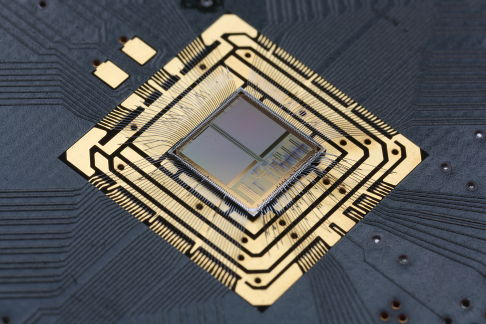
\includegraphics[width=0.75\textwidth]{media/spikey_chip_small.jpg}\\[0.25cm]
			\footnotesize\textcolor{aluminium4}{Spikey Neuromorphic Chip\\ Source: Electronic Visions Group, KIP Heidelberg}
			\column{0.5\textwidth}
			\centering
			\textcolor{violet}{\addfontfeatures{LetterSpace=2.5}COMPUTATIONAL NEUROSCIENCE}\\\emph{Build biologically constrained models of cognition}\\[0.25cm]
			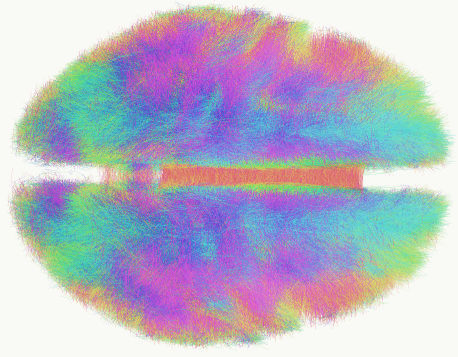
\includegraphics[height=3.5cm]{media/connectome.jpg}\\[0.25cm]	\footnotesize\textcolor{aluminium4}{Human Connectome. Data by Horn A.~et al., 2014\\ Source: Wikimedia Commons}
		\end{columns}
	\end{overlayarea}
\end{frame}
\backupend

\end{document}
